\section{度量熵}

对于次高斯

在度量空间理论中, $\epsilon$-网,  $\epsilon$-覆盖, 

ε网、ε包、ε覆盖、均匀离散集、相对密集集和德尔尼集(以鲍里斯·德尔尼命名)是几个紧密相关的定义,用于描述点集的良好分布,这些集合的包络半径和覆盖半径衡量了它们的分布情况。
这些集合在编码、近似算法等理论中有着应用. 


度量空间$(\cX, \rho)$的子集$T$



\begin{figure}[H]
	\centering 
	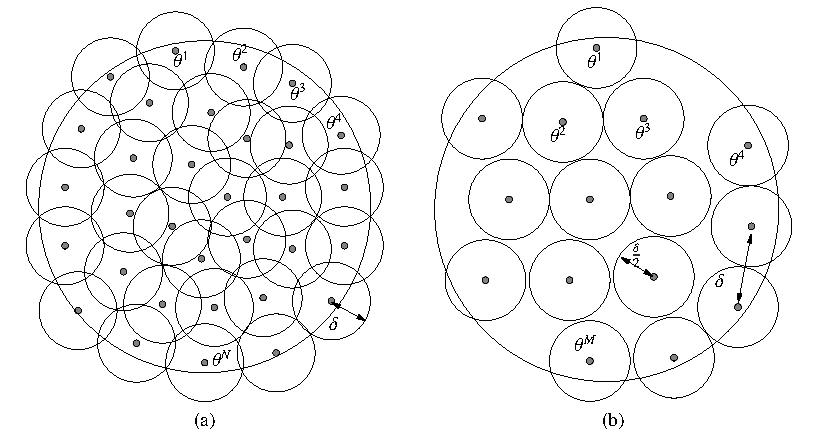
\includegraphics[width=.95\textwidth]{figure/covering-packing.pdf}
\end{figure}


\begin{figure}[H]
	\centering 
	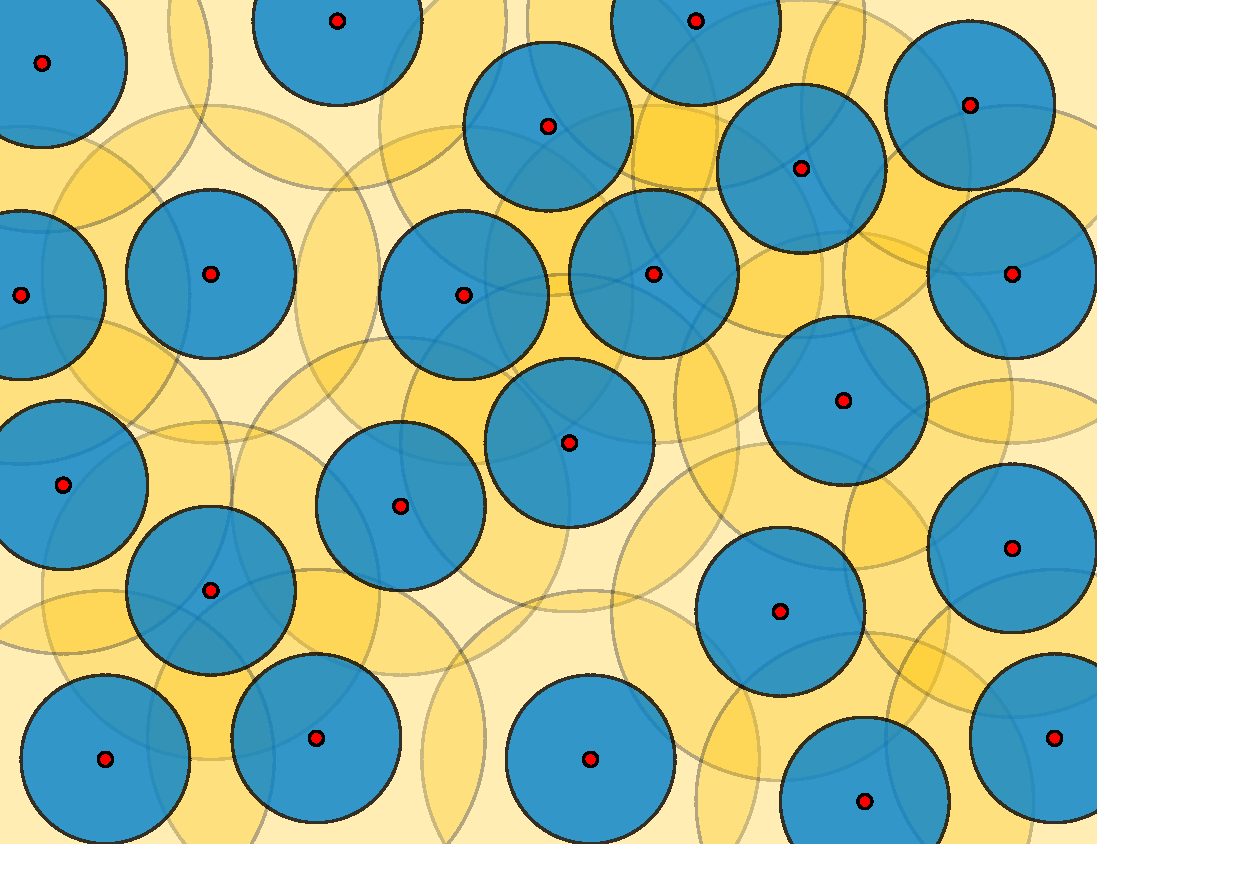
\includegraphics[width=.5\textwidth]{figure/Metric_epsilon-net.pdf}
\end{figure}







